% SIAM Article Template
\documentclass[review,onefignum,onetabnum]{siamart190516}

% Information that is shared between the article and the supplement
% (title and author information, macros, packages, etc.) goes into
% ex_shared.tex. If there is no supplement, this file can be included
% directly.
\usepackage{subfig}
\usepackage{multirow}
\usepackage{textcomp}
\usepackage{stmaryrd}
\usepackage{boldfonts}
\usepackage{symbols}
\usepackage{lipsum}
\usepackage{amsfonts}
\usepackage{graphics}
\usepackage{graphicx}
\usepackage{epstopdf}
\usepackage{algorithmic}
\usepackage{diagbox}
\usepackage{mathtools}
\usepackage{tikz}
\ifpdf
  \DeclareGraphicsExtensions{.eps,.pdf,.png,.jpg}
\else
  \DeclareGraphicsExtensions{.eps}
\fi

% Add a serial/Oxford comma by default.
\newcommand{\creflastconjunction}{, and~}

% Used for creating new theorem and remark environments
\newsiamremark{remark}{Remark}
\newsiamremark{hypothesis}{Hypothesis}
\crefname{hypothesis}{Hypothesis}{Hypotheses}
\newsiamthm{claim}{Claim}

% Sets running headers as well as PDF title and authors
\headers{Choice of interior penalty coefficient for DG
for Biot's system by employing machine learning}{S. Lee, T. Kadeethum, H. M. Nick}

% Title. If the supplement option is on, then "Supplementary Material"
% is automatically inserted before the title.
\title{Choice of interior penalty coefficient for interior penalty discontinuous Galerkin method for Biot's system by employing machine learning\thanks{Submitted to the editors DATE.
\funding{This work was funded by XXX.}}}

% Authors: full names plus addresses.
\author{Sanghyun Lee\thanks{Department of Mathematics, Florida State University
  (\email{lee@math.fsu.edu}, \url{http://https://www.math.fsu.edu/\string~lee/}).}
\and Teeratorn Kadeethum\thanks{Technical University of Denmark, 
  (\email{teekad@dtu.dk}, \email{hamid@dtu.dk}).}
\and Hamid M. Nick\footnotemark[3]}

\usepackage{amsopn}
\DeclareMathOperator{\diag}{diag}


\usepackage{eqnarray}

\newcommand{\shlee}[1]{{\textcolor{blue}{#1}}}
\newcommand{\bdf}[2]{{\textup{\textsf{BDF}}_{#2}\left({#1}\right)}}
\newcommand{\BDF}[1]{\bdf{\left( #1 \right)}{2}}

\newcommand{\vertiii}[1]{{\left\vert\kern-0.25ex\left\vert\kern-0.25ex\left\vert #1 
    \right\vert\kern-0.25ex\right\vert\kern-0.25ex\right\vert}}
\def\p{\partial}


% Optional PDF information
\ifpdf
\hypersetup{
  pdftitle={Choice of interior penalty coefficient for interior penalty discontinuous Galerkin method  by employing machine learning},
  pdfauthor={S.Lee, T. Kadeethum, Nick H}
}
\fi

% The next statement enables references to information in the
% supplement. See the xr-hyperref package for details.

%\externaldocument{ex_supplement}

% FundRef data to be entered by SIAM
%<funding-group specific-use="FundRef">
%<award-group>
%<funding-source>
%<named-content content-type="funder-name"> 
%</named-content> 
%<named-content content-type="funder-identifier"> 
%</named-content>
%</funding-source>
%<award-id> </award-id>
%</award-group>
%</funding-group>

\begin{document}

\maketitle

% REQUIRED
\begin{abstract}
  In this paper, optimal choice of the interior penalty parameter for the elliptic problems and the Biot's systems are studied by utilizing the neural network and machine learning. 
\end{abstract}

% REQUIRED
\begin{keywords}
Discontinuous Galerkin, Interior Penalty, Neural Network, Machine Learning, Finite Element Methods
\end{keywords}

% REQUIRED
\begin{AMS}
  68Q25, 68R10, 68U05
\end{AMS}

\section{Introduction}

Discontinuous Galerkin finite element method (DG) is one of the most popular non conforming finite elements  employed for various realistic applications, especially with discontinuous coefficients. The idea of DG finite element methods originated from  [74]  and extended by several authors including 
[38,118,84,4], which were so called Interior Penalty Galerkin Methods.  
Perhaps, the most popular and successful methods in terms of the local flux conservation is DG. 
DG can deal robustly with general partial differential equations as well as with equations whose 
type changes within the computational domain 
such as from advection dominated to diffusion dominated \cite{Sun2005, Sun2006}. [77] 
They are naturally suited for multi-physics applications, and for problems with highly varying material properties \cite{ref1,riviere2000discontinuous,CNM:CNM464}.  [26,28]

However, one of the main disadvantage of DG is that the stability and the accuracy of the scheme depends on the interior penalty  parameter that needs to be chosen. 
These numerical analyses of DG are proved under an assumption on the interior penalty parameter, and it is crucial to employ the optimal interior penalty parameter. 
Generally, if the parameter is too large, DG schemes converge to the continuous Galerkin finite element methods, and ofter suffer from the linear solver. If the parameter is too small, the stability of the scheme is not guaranteed. 


Thus, several studies of the lower bounds for the penalty parameter have been obtained in \cite{ainsworth2007posteriori,ainsworth2010fully,ainsworth2009constant,epshteyn2007estimation,shahbazi2005explicit}. 
A lower boundary for the interior penalty parameter for arbitrary nonuniform polynomial order was first shown in 
 \cite{shahbazi2005explicit} and it was improved in \cite{ainsworth2009constant} by assuming at most one hanging node per edge of each element. In \cite{ern2008posteriori,ern2009discontinuous}, a weighted interior penalty parameters for the cases where the diffusion coefficient is discontinuous were studied. 
Moreover, specific illustrations on the selection of the penalty parameters are shown in \cite{ainsworth2012note}.

In this paper, we propose the method to find the optimal interior penalty parameters for both elliptic problems and the poroelasitic Biot system. However, the novelty in our paper is that we employ the neural networks and machine learning processes. 
\shlee{We need to discuss about the machine learning algorithm / neural networks here.}
When various numerical simulations are necessary, 
but with different numerical and physical parameters (e.g mesh size, permeability, viscosity, etc), 
this computational framework could be very efficient and robust. 

% The outline is not required, but we show an example here.
The paper is organized as follows. Our governing system and finite element discretizations  are in
\cref{sec:main}. Details about the machine learning algorithm is discussed  in \cref{sec:alg}.  Finally, numerical results are in \cref{sec:experiments}, and the conclusions follow in
\cref{sec:conclusions}.





\section{Mathematical Model}
\label{sec:main}


In this section, we briefly recapitulate the Biot system for poro-elasticity that we will discuss in this paper.  
Let $\Omega \subset \mathbb{R}^d$ ($d \in \{1,2,3\}$) be the computational domain, which is bounded by the boundary, $\partial \Omega$. The time domain is denoted by $\mathbb{T} = \left(0,T\right]$ with $T>0$. 
Then the coupling between the fluid flow and solid deformation can be captured through the application of Biot\textquotesingle s equation of poroelasticity, which is composed of linear momentum and mass balance equations \cite{biot1941general}.

First, the mass balance equation is given as \cite{coussy2004poromechanics}:
%%%%%
\begin{equation} \label{eq:mass_balance}
\rho\left(\phi c_{f}+\dfrac{\alpha-\phi}{K_{s}}\right) \dfrac{\partial}{\partial t}p + 
\rho \alpha \frac{\partial}{\partial t} \nabla \cdot \bu -
\nabla \cdot \bkappa(\nabla p-\rho \mathbf{g})=g \text { in } \Omega \times \mathbb{T},
\end{equation}
where 
$p(\cdot ,  t) : \Omega \times  (0; T] \to \mathbb{R}$  
is a scalar-valued fluid pressure, 
$\mathbf{u} (\cdot , t) : \Omega \times  (0; T] \to \mathbb{R}^d$ 
is a vector-valued displacement,
$\rho$ is a fluid density, $\phi$ is an initial porosity, 
$c_f$ is a fluid compressibility, $\bg$ is a gravitational vector, $g$ is a sink/source.
Here, $\nabla \cdot \bu$ term represents the volumetric deformation and $\bkappa$ is defined as:
%%%
\begin{equation}
\bkappa:=\frac{\rho {\bk_{m}}}{\mu}, 
\label{eq:kappa}
\end{equation}
%%%
where $\bk_m$ is a matrix permeability tensor and $\mu$ is a fluid viscosity. By assuming that the rock volumetric displacement can cause the matrix permeability alteration, $\bk_{m}$ is defined as \cite{abou2013petroleum,Du2007}:
%%%%
\begin{equation}\label{eq:wong_perm}
\bk_{m}=\bk_{m_0}\dfrac{\left(1+\dfrac{\varepsilon_{v}}{\phi}\right)^{3}}{1+\varepsilon_{v}},
\end{equation}
%%%
where $\bk_{m_0}$ represent an initial rock matrix permeability. Here, $\varepsilon_{v}$ is the total volumetric strain, which is defined as:
%%%%
\begin{equation} \label{eq:volumetric_str}
\varepsilon_{v} :=\operatorname{tr}({\bepsilon(\bu)})=\sum_{i=1}^{d} \bepsilon(\bu)_{i i},
\end{equation}
%%%%
where 
$\bepsilon(\bu)$ is a strain,  which is  defined as:
%%%%%
\begin{equation}
\bepsilon(\bu) :=\frac{1}{2}\left(\nabla \bu+\nabla \bu^{T}\right),
\end{equation}
by assuming infinitesimal displacements. 
Throughout this paper, we assume $\rho$ and $\mu$ are constants but  $\bkappa$ varies as a function of $\bk_m$. 

The mass balance equation (the fluid flow problem) is supplemented by the following boundary and initial conditions: 
%%%%%
\begin{eqnarray}
p&=&p_{D} \text { on } \partial \Omega_{p} \times \mathbb{T}, \\
-\nabla \cdot \bkappa(\nabla p-\rho \mathbf{g}) \cdot \bn&=&q_{D} \text { on } \partial \Omega_{q} \times \mathbb{T}, \\
p&=&p_{0} \text { in } \Omega \text { at } t = 0,
\end{eqnarray}
where $p_D$ and $q_D$ are specified pressure and flux, respectively,
and $\partial \Omega$ is decomposed to pressure and flux boundaries, $\partial \Omega_p$ and $\partial \Omega_q$, respectively.



Secondly, the linear momentum balance equation can be written as follows: 
\begin{equation}
\nabla \cdot \bsigma (\bu,p) =\bf{f}.
\end{equation}
For the simplicity,  a body force $\bf{f}$ is neglected in this study.  Here, $\bsigma$ is total stress, which is defined as:
%%%
\begin{equation}
\bsigma := \bsigma(\bu, p) = \bsigma^{\prime}(\bu) - \alpha p \bI,
\end{equation}
%%%
where $\bI$ is the identity tensor and $\alpha$ is Biot\textquotesingle s coefficient defined as \cite{Jaeger2010}:
%%%%
\begin{equation} \label{eq:biot_coeff}
\alpha:=1-\frac{K}{K_{{s}}},
\end{equation}
%%%%
with the bulk modulus of a rock matrix $K$ and the solid grains modulus $K_s$. In addition, $\bsigma^{\prime}$ is an effective stress written as: 
%%%%
\begin{equation}
\bsigma^{\prime}:= \bsigma^{\prime}(\bu) = 
2 \mu_{l} \bepsilon(\bu)-\lambda_{l} \nabla \cdot \bu \bI,
\end{equation}
%%%%
where $\lambda_{l}$ and $\mu_{l}$ are Lam\'e constants.
%%%%%
Thus, we can write the linear momentum balance supplemented by its boundary and initial conditions as:
%%%%%%
\begin{eqnarray}
\label{eq:linear_balance}
\nabla \cdot \bsigma^{\prime}(\bu) +\alpha \nabla \cdot p \bI 
&= &\bf{f} \hspace{0.14in} \text { in } \Omega \times \mathbb{T}, \\
\bu &=&\bu_{D} \text { on } \partial \Omega_{u} \times \mathbb{T},\\
\bsigma^{\prime} \cdot \bn&=&\bsigma_{D} \text { on } \partial \Omega_{t} \times \mathbb{T}, \\
\bu&=&\bu_{0} \hspace{0.06in} \text { in } \Omega \text { at } t = 0,
\end{eqnarray}
where $\bu_D$ and ${\bsigma_D}$ are prescribed displacement and traction at boundaries, respectively, and $t$ is time.
Here, $\partial \Omega$ can be decomposed to displacement and traction boundaries, $\partial \Omega_u$ and $\partial \Omega_t$, respectively, for the solid deformation problem. 




\section{Numerical Discretizations}

For this paper, we employ the discontnious Galerkin (DG) finite element method for the spatial discretization. Let $\mathcal{T}_h$ be the shape-regular (in the sense of Ciarlet)  triangulation by a family of partitions of $\O$ into $d$-simplices $\K$ (triangles/squares in $d=2$ or tetrahedra/cubes in $d=3$). We denote by $h_{\K}$ the diameter of $\K$ and we set $h=\max_{\K \in \Th} h_{\K}$.  
Also we denote by $\Eh$ the set of all edges and by $\Eho$ and $\Ehb$ the collection of all interior and boundary edges, respectively. 
In the following notation, we assume edges for two dimension but the results hold analogously for faces in three dimensional case.
The space $H^{s}(\Th)$ $(s\in \mathbb{R})$ is the set of element-wise $H^{s}$ functions on $\mathcal{T}_h$, and $L^{2}(\Eh)$ refers to the set of functions whose traces on the elements of $\Eh$ are square integrable. Let $\mathbb{Q}_l(\K)$ denote the space of polynomials of partial degree at most $l$. 
Throughout the paper, we use the standard notation for Sobolev spaces and their norms. For example, let $E \subseteq \Omega$, then $\|\cdot\|_{1,E}$ and $|\cdot|_{1,E}$ denote the $H^1(E)$ norm and seminorm, respectively. 
For simplicity, we eliminate the subscripts on the norms if $E = \Omega$.

Since we consider the nonconforming DG methods, 
let
$$
e = \partial \K^{+}\cap \partial \K^{-}, \ \ e \in \Eho,
$$
where  $\K^{+}$ and $\K^{-}$ be two neighboring elements 
and we denote by $h_{e}$ the length of the edge $e$. 
Let $\n^{+}$ and $\n^{-}$ be the outward normal unit vectors to  $\partial T^+$ and $\partial T^-$, respectively ($\n^{\pm} :=\n_{|\K^{\pm}}$). 
For any given function $\xi$ and vector function $\bxi$, defined on the triangulation $\mathcal{T}_h$, we denote $\xi^{\pm}$ and $\bxi^{\pm}$ by the restrictions of $\xi$ and $\bxi$ to $T^\pm$, respectively. 

Next, we define the weighted average operator
$\{\cdot \}_{\delta_{e}}$  as follows:
for $\zeta \in L^2(\mathcal{T}_h)$ and $\taub \in L^2(\mathcal{T}_h)^d$,
\begin{equation}
\{\zeta\}_{\delta e}=\delta_{e} \zeta^{+}+\left(1-\delta_{e}\right) \zeta^{-}, \ \text{ and } \ 
\{\taub\}_{\delta e}=\delta_{e} \taub^{+}+\left(1-\delta_{e}\right) \taub^{-},
\ \text{ on } e \in \Eho,
\end{equation}
where $\delta_{e}$ is calculated by \cite{ErnA_StephansenA_ZuninoP-2009aa,ern2008posteriori}.
\begin{equation}
\delta_{e} :=\frac{{\kappa}^{-}_e}{{\kappa}^{+}_e+{\kappa}^{-}_e}.
\end{equation}
Here, 
\begin{equation}
{\kappa}^{+}_e :=\left(\bn^{+}\right)^{T} \cdot \bkappa^{+} \cdot \bn^{+}, \ \text{ and }
{\kappa}^{-}_e :=\left(\bn^{-}\right)^{T} \cdot \bkappa^{-} \cdot \bn^{-},
\end{equation}
where  ${\kappa_e}$ is a harmonic average of $\kappa^{+}_e$ and ${\kappa}^{-}_e$ read as:
\begin{equation}
{\kappa_{e}}:= \frac{2{\kappa}^{+}_e {\kappa}^{-}_e}{\left({\kappa}^{+}_e+{\kappa}^{-}_e\right)}.
\end{equation}
%%%
On the other hand, for $e \in \Ehb$, we set $\av{\zeta}_{\delta_e} :=   \zeta$ and $\av{\taub}_{\delta_e} :=  \taub$. 
The jump across the interior edge will be defined as 
\begin{align*}
\jump{\zeta} = \zeta^+\n^++\zeta^-\n^- \quad \mbox{ and } \quad \jtau = \taub^+\cdot\n^+ + \taub^-\cdot\n^- \quad \mbox{on } e\in \Eho. 
\end{align*}
For  $e \in \Ehb$, we let $\jump{\zeta} :=  \zeta \bn$ and $\jump{\taub} :=  \taub \cdot \bn$. 

Finally, we introduce 
the finite element space for the discontinuous Galerkin method, which is the space of piecewise discontinuous polynomials of degree $k$ by
\begin{equation}
V^{\textsf{DG}}_{h,k} (\mathcal{T}_h) := \left \{ \psi \in L^2(\Omega) | \ \psi_{|_{\K}} \in \mathbb{Q}_k(\K), \ \forall \K \in \mathcal{T}_h \right \}.
\end{equation}
%%%%%%%%%%%%%%%%
Moreover, we use the notation: 
\begin{align*}
&(v,w)_{\Th}:=\dyle\sum_{\K \in \Th} \int_{\K} v\, w dx, \quad \forall\,\, v ,w \in L^{2} (\mathcal{T}_h), \\
&\langle v, w\rangle_{\Eh}:=\dyle\sum_{e\in \Eh} \int_{e} v\, w \,d\gamma, \quad \forall\, v, w \in L^{2}(\Eh).
\end{align*}
%%%%%%%%%%%%%%%%%%% 

\subsection{Pressure equation}

First, we introduce the backward Euler DG approximation to \eqref{eq:mass_balance}. 
We define a partition of the time interval $0=:t^0 <t^1 < \cdots <  t^N := \mathbb{T} $ and denote the uniform time step size by $\delta t:= t^n - t^{n-1}$.
The DG finite element space approximation of the pressure $p(\bx,t)$ is denoted by $P(\bx,t) \in V^{DG}_{h,k}$. 
Let $P^n := P(\bx,t^n)$ for  $0 \leq n \leq N$. 
We set a given initial condition for the pressure as $P^0$ and assume the displacement at time $t$, $\bu(\cdot,t)$ is given.
\shlee{For the simplicity the gravity and the source/sink terms are neglected.}
Then, the time stepping algorithm reads as follows: Given $P^{n-1}$, 
\begin{equation}\label{eq:dgscheme}
\mbox{ Find  }P^{n} \in V_{h,k}^{DG} \mbox{  such that  } \calS_\theta(P^{n},w) = \mathcal{F}_\theta(w), \quad \forall\, w\in V_{h,k}^{DG}, \,
\end{equation}
where $\calS_\theta$ and $\mathcal{F}_\theta$ are the bilinear form and linear functional as defined by
\begin{multline}\label{stheta}  
\calS_{\theta}(v,w) :=
\dfrac{\rho}{\delta t}\left(\phi c_{f}+\frac{\alpha-\phi}{K_{s}}\right) \left ( v, w \right)_{\Th} \\
+ \left (\bkappa \nabla v,\nabla w \right )_{\Th} 
- \left \langle \av{ \bkappa \nabla v }_{\delta_{e}}, \jump{w} \right \rangle_{\mathcal{E}_h^{1}} \\
 - \theta \left \langle \jump{v},\av{ \bkappa \nabla w}_{\delta_{e}} \right \rangle_{\mathcal{E}_h^{1}} + \beta(k)  \langle h^{-1}_{e}  \kappa_e \jump{v},\jump{w} \rangle_{\mathcal{E}_h^{1}}, 
\quad \forall v, w \in V_{h,k}^{DG},  
\end{multline}
and 
\begin{multline}
\mathcal{F}_\theta(w) := \frac{1}{\delta t}(P^{n-1}, w)_{\mathcal{T}_h} 
- \rho \alpha(\dfrac{\partial}{\partial t} \nabla \cdot \bu,w)_{\mathcal{T}_h} 
- \left \langle  {q_D},\jump{w} \right \rangle_{\mathcal{E}_h^{N,\partial}} \label{ftheta} \\
\quad - \theta \left \langle p_D,\av{ \bkappa \nabla w}_{\delta_{e}} \right \rangle_{\mathcal{E}_h^{D,\partial}} 
+ \beta(k)  \langle h^{-1}_{e} \kappa_e p_D,\jump{w}\rangle_{\mathcal{E}_h^{D,\partial}},
\quad \forall w \in V_{h,k}^{DG}.
\end{multline}



({\color{blue} see Luigi's thesis to clarify the reference})
 The {choice} of $\theta$ leads to different DG algorithms. For example, i) $\theta = 1$ for SIPG($\beta$)$-k$ methods \cite{StenbergR-1998aa,Dryja2003}, which later has been extended to the advection-diffusion problems in \cite{BurmanE_ZuninoP-2006aa,Di-PietroD_ErnA_GuermondJ-2008aa},
ii) $\theta = -1$ for NIPG($\beta$)$-k$ methods \cite{HoustonP_SchwabC_SuliE-2002aa}, and iii) $\theta = 0$ for IIPG($\beta$)$-k$ method \cite{DawsonC_SunS_WheelerM-2004aa}.

The interior penalty parameter, $\beta(k)$, is a function of polynomial degree approximation, $k$. Here, $h_e$ is a characteristic length of the edge $e \in \Eh$ calculated as:
\begin{equation}
h_{e} :=\frac{\operatorname{meas}\left(T^{+}\right)+\operatorname{meas}\left(T^{-}\right)}{2 \operatorname{meas}(e)},
\end{equation}
where meas($.$) represents a measurement operator, measuring length, area, or volume. Several analysis for the choice of the interior penalty parameter are shown in [X] and this $\beta$ is the quantatiy 
that we investigate in this paper. 


\subsection{Poroelasticity problem}

For the displacement $\bu$, we employ the classical continuous Galerkin (CG)finite element methods for the spatial discretizations as in \cite{choo2018enriched,Kadeethum2019} where the function space is defined as 
\begin{equation}
W^{\textsf{CG}}_{h,k} (\mathcal{T}_h) :=
\left\{\bpsi_u \in \mathbb{C}^{0}(\Omega{; \mathbb{R}^d}) :\left.\bpsi_u \right|_{T} \in \mathbb{Q}_{k}(T{; \mathbb{R}^d}), \forall T \in \mathcal{T}_{h}\right\},
\label{eq:CG_U}
\end{equation}
where
$\mathbb{C}^0(\Omega{; \mathbb{R}^d})$ denotes the space of vector-valued piecewise continuous polynomials, $\mathbb{Q}_{k}(T{; \mathbb{R}^d})$ is the space of polynomials of degree at most $k$ over each element $T$.


The CG finite element space approximation of the displacement $\bu(\bx,t)$ is denoted by $\bU(\bx,t) \in W^{CG}_{h,k}$. 
Let $\bU^n := \bU(\bx,t^n)$ for  $0 \leq n \leq N$. 
We set a given initial condition for the pressure as $\bU^0$ and the pressure at time $t$, $P^n$ is given from the previous section.
%%%%%
Then, the time stepping algorithm reads as follows: Given $\P^{n}$, 
\begin{equation}\label{eq:cgscheme}
\mbox{ Find  } \bU^{n} \in W_{h,k}^{CG} \mbox{  such that  } \calA(\bU^{n},\bw) = \mathcal{D}(\bw), \quad \forall\, \bw\in W_{h,k}^{CG}, \,
\end{equation}
where $\calA$ and $\mathcal{D}$ are the bilinear form and linear functional as defined as 
\begin{equation}\label{Dtheta}  
\calA(\bv,\bw) :=
\sum_{T \in \mathcal{T}_{h}} \int_{T}
\bsigma^{\prime}\left(\bv \right) : \nabla^{s} \bw \: d V  +  \sum_{T \in \mathcal{T}_{h}} \int_{T} \alpha  \nabla P^n  . \nabla \bw \: d V,
\quad \forall\, \bv, \bw\in W_{h,k}^{CG},
\end{equation}
and 
\begin{equation}
\mathcal{D}(\bw) :=
\sum_{T \in \mathcal{T}_{h}} \int_{T} {\bf{f}} \bw \: d V
+\sum_{e \in \mathcal{E}_{h}^{N}} \int_{e} \bsigma_D \bw \: d S, 
\quad \forall\, \bw\in W_{h,k}^{CG},
\end{equation}


\section{Machine Learning Algorithm}
\label{sec:alg}

In this section, we discuss the details for the neural network and machine learning algorithm that we employ for our numerical scheme to find the optimal choice of interior penalty parameter. 
The overall algorithm is based on [x]




Our analysis leads to the algorithm in \cref{alg:buildtree}.
\begin{algorithm}
\caption{Build tree}
\label{alg:buildtree}
\begin{algorithmic}
\STATE{Define $P:=T:=\{ \{1\},\ldots,\{d\}$\}}
\WHILE{$\#P > 1$}
\STATE{Choose $C^\prime\in\mathcal{C}_p(P)$ with $C^\prime := \operatorname{argmin}_{C\in\mathcal{C}_p(P)} \varrho(C)$}
\STATE{Find an optimal partition tree $T_{C^\prime}$ }
\STATE{Update $P := (P{\setminus} C^\prime) \cup \{ \bigcup_{t\in C^\prime} t \}$}
\STATE{Update $T := T \cup \{ \bigcup_{t\in\tau} t : \tau\in T_{C^\prime}{\setminus} \mathcal{L}(T_{C^\prime})\}$}
\ENDWHILE
\RETURN $T$
\end{algorithmic}
\end{algorithm}



\section{Numerical results}
\label{sec:experiments}

In this section, several numerical examples are illustrated to show the capability of our proposed algorithm and computational framework.

\subsection{Elliptic Problems}
First, we consider the simplified equation of the flow problems 
\eqref{eq:mass_balance}.
By assuming that the pressure doesn't depend on the time and $\bu$ is a given constant, we obtain 
\begin{equation} \label{eq:mass_balance_elliptic}
-\nabla \cdot ( \bkappa \nabla p)= g \text { in } \Omega \times \mathbb{T}. 
\end{equation}
Moreover, we note that the gravity ($\bg$) and the source/sink term (g) are neglected for the simplicity. 

\subsubsection{The effect of a polynomial degree approximation ($k$)} We investigate the effect of a polynomial degree approximation on the choice of optimal $\beta$ using different solvers and discretization schemes. We study five $k$ values (1, 2, 3, 4, and 5) and use Algorithm \ref{alg:ell_effect_of_k} for each case, i.e. each case has different combination of solver, discretization, and $k$. 

\begin{algorithm}[!ht]
\caption{Investigation procedure for the elliptic problem}
\label{alg:ell_effect_of_k}
\begin{algorithmic}
\STATE{Initialize the set of $\boldsymbol{\kappa}$ that used in the investigation}
\FOR{$i$ $<$ $n_{\boldsymbol{\kappa}}$, where $n_{\boldsymbol{\kappa}}$ is the size of the specified $\boldsymbol{\kappa}$ list}
\STATE{Assign $\boldsymbol{\kappa}:=\boldsymbol{\kappa}\left[i\right]$}
\STATE{Assign $\beta:=\beta_0$, where $\beta_0 = 100.00$}
\STATE{Initialize error convergence rate list, where all members = $k$}
\WHILE{$\forall$ error convergence rate $\in$ error convergence rate list = $\left[ k - \epsilon, k + \epsilon \right]$, where $\epsilon = 0.5 \times k$}
\STATE{Clear error convergence rate list}
\STATE{Assign $h:=h_0$, where $h_0 = $}
\STATE{Update $\beta:=0.99 \times \beta$} \COMMENT{Except the first loop}
\FOR{$j$ $<$ $n_h$, where $n_h = 6$}
\STATE{Calculate $H_0^1$ norm}
\STATE{Calculate error convergence rate}
\STATE{Append error convergence rate list}
\STATE{Update $h:=0.5 \times h$}
\ENDFOR
\ENDWHILE
\RETURN $\beta$, this $\beta$ is the smallest $\beta$, which the optimal error convergence rate can be observed.
\ENDFOR
\end{algorithmic}
\end{algorithm}

We take $\Omega = \left[ 0,1\right]^2$ and choose the exact solution in $\Omega$ as:

\begin{equation}\label{eq:darcy_exact_solution}
p(x,y) := \sin(x+y),
\end{equation}

\noindent
where $x$ and $y$ represent points in x- and y-direction, respectively, and $\boldsymbol{\kappa}$ is read: 

\begin{equation}\label{eq:darcy_exact_solution_kappa}
\boldsymbol{\kappa} := \kappa  \boldsymbol{I},
\end{equation}

\noindent
where $\kappa$ represents a multiplied coefficient in a range of $[1.0,1 \times 10^{-18}]$ for the whole domain, and $\boldsymbol{I}$ is an identity matrix. Subsequently, $g$ is chosen as: 

\begin{equation}  \label{eq:darcy_source}
g(x,y) := 2.0\cos(x+y)
\end{equation}

\noindent
to satisfy the exact solution. Furthermore, the homogeneous boundary conditions are applied to all boundaries using Equation~(\ref{eq:darcy_exact_solution}). The results are presented in Table \ref{tab:ell_homo_beta_unstable}, and it shows that the lowest $\beta$ values of SIPG are higher than those of IIPG. Besides, the type of solver, direct and iterative solvers, does not influence this value, and the smallest $\beta$ increases as $k$ increases. 

\begin{table}[!ht]
  \centering
  \caption{The lowest $\beta$ value that provides the optimal error convergence rate solution with different $k$, discretization, and solver. Note that $\boldsymbol{{\kappa}}$ is homogeneous.}
    \begin{tabular}{|c|c|c|c|c|}
    \hline
    \multirow{2}[4]{*}{$k$} & \multicolumn{2}{c|}{SIPG} & \multicolumn{2}{c|}{IIPG} \\
\cline{2-5}          & \multicolumn{1}{l|}{direct solver} & \multicolumn{1}{l|}{iterative solver} & \multicolumn{1}{l|}{direct solver} & \multicolumn{1}{l|}{iterative solver} \\
    \hline
    1     & 1.11  & 1.11  & 0.83  & 0.83 \\
    \hline
    2     & 2.80  & 2.80  & 2.74  & 2.74 \\
    \hline
    3     & 5.79  & 5.79  & 5.68  & 5.68 \\
    \hline
    4     & 9.99  & 9.99  & 9.79  & 9.79 \\
    \hline
    5     & 14.97 & 14.97 & 14.67 & 14.67 \\
    \hline
    \end{tabular}%
  \label{tab:ell_homo_beta_unstable}%
\end{table}%

The choice of $\beta$, however, impacts the number of linear iterative solver significantly, as presented in Figures \ref{fig:ell_homo_sipg_noi} and \ref{fig:ell_homo_iipg_noi} for SIPG and IIPG results, respectively. As one observes, when $\beta$ is increased, the number of iteration increases. On the other hand, when $\beta$ is approaching zero, the number of iteration, again, increases dramatically; and subsequently, the solution becomes unstable. Hence, the choice of $\beta$ is essential because if we select a large value of $\beta$, our simulation takes more time to converge, while a small value can also cause the higher number of iteration and more importantly unstable solution.

\begin{figure}[h!]
   \centering
        \includegraphics[width=6.0cm, height=6.0cm]{pictures/ell_homo_diff_k_sipg_it_k1.pdf}
        \includegraphics[width=6.0cm, height=6.0cm]{pictures/ell_homo_diff_k_sipg_it_k2.pdf}
        \includegraphics[width=6.0cm, height=6.0cm]{pictures/ell_homo_diff_k_sipg_it_k3.pdf}
        \includegraphics[width=6.0cm, height=6.0cm]{pictures/ell_homo_diff_k_sipg_it_k4.pdf}
        \includegraphics[width=6.0cm, height=6.0cm]{pictures/ell_homo_diff_k_sipg_it_k5.pdf}
   \caption{Number of linear iterative solver of SIPG for (\textbf{a}) $k=1$, (\textbf{b}) $k=2$, (\textbf{c}) $k=3$, (\textbf{d}) $k=4$, and (\textbf{e}) $k=5$. Note that each line represents different value of ${\kappa}$, and the error bar shows mean and standard derivation of each number of iteration.}
   \label{fig:ell_homo_sipg_noi}
\end{figure}

\begin{figure}[h!]
   \centering
        \includegraphics[width=6.0cm, height=6.0cm]{pictures/ell_homo_diff_k_iipg_it_k1.pdf}
        \includegraphics[width=6.0cm, height=6.0cm]{pictures/ell_homo_diff_k_iipg_it_k2.pdf}
        \includegraphics[width=6.0cm, height=6.0cm]{pictures/ell_homo_diff_k_iipg_it_k3.pdf}
        \includegraphics[width=6.0cm, height=6.0cm]{pictures/ell_homo_diff_k_iipg_it_k4.pdf}
        \includegraphics[width=6.0cm, height=6.0cm]{pictures/ell_homo_diff_k_iipg_it_k5.pdf}
   \caption{Number of linear iterative solver of IIPG for (\textbf{a}) $k=1$, (\textbf{b}) $k=2$, (\textbf{c}) $k=3$, (\textbf{d}) $k=4$, and (\textbf{e}) $k=5$. Note that each line represents different value of ${\kappa}$, and the error bar shows mean and standard derivation of each number of iteration.}
   \label{fig:ell_homo_iipg_noi}
\end{figure}

To predict the optimal $\beta$ for the iterative solver, i.e., requires minimum linear solver iteration and provides stable solutions, we firstly identify the parameters, which impact the number of iteration (dependent variable). The chi-squared test \cite{scikit-learn} is performed, and its results are provided in Table \ref{tab:linear_regression_p_value}. From this table, $\theta$, $\beta$, $h$, and $k$ have a p-value less than 0.025; therefore, we include these variables as independent variables for a further predictive model development. 

\begin{table}[!ht]
  \centering
  \caption{Elliptic equation with continuous exact solution: p-value results for each explanatory variable}
    \begin{tabular}{|c|c|}
    \hline
    Variable & p-value \\
    \hline
    $\theta$ & $\approx$ 0.00 \\
    \hline
    $\kappa$ & $\approx$ 1.00 \\
    \hline
    $\beta$  & $\approx$ 0.00 \\
    \hline
    $h$     & $\approx$ 0.00 \\
    \hline
    $k$     & $\approx$ 0.00 \\
    \hline
    \end{tabular}%
  \label{tab:linear_regression_p_value}%
\end{table}%

In total, we have TODO data points and split training, validation, and test sets uniformly \cite{scikit-learn} using $\left[ 0.8, 0.1 ,0.1\right]$ splitting ratio. We use training set to train the multi-variable regression and ANN models, validation set for hyper-parameter tuning for the ANN model, and test set for comparison performances between the multi-variable regression and ANN model. We begin with building the multi-variable regression \cite{scikit-learn} as follows:

\begin{remark}
\shlee{
The reason that $\kappa$ does not effect the results: existence of $\kappa$ as a coefficient of the penalty term. }
\end{remark}

\begin{equation} \label{eq:ell_regression_con}
\begin{split}
\mathrm{number \ of \ iteration} = \alpha 
    &+ \gamma_{1} \times \theta \\
    &+ \gamma_{2} \times \beta    \\
    &+ \gamma_{3} \times h \\
    &+ \gamma_{4} \times k
\end{split}
\end{equation}

\noindent
where $\alpha = 16.93$, $\gamma_{1} = -1.11$, , $\gamma_{2} = 0.21$, , $\gamma_{3} = -9.85$, and $\gamma_{4} = 0.02$. The $r^2$ and explained variance score is 0.60 and 0.60, respectively.

Subsequently, we develop ANN model using four input and one output as presented in Figure \ref{fig:ell_ann_fig} and use number of hidden layer ($n_{hl}$) and number of neuron ($n_n$) for hyper-parameter tuning. For the sake of simplicity we assume each hidden layer has the same number of neuron. Rectified Linear Unit (ReLU) is used as an activation function for each neuron of the hidden layer. 

\tikzset{%
  every neuron/.style={
    circle,
    draw,
    minimum size=1cm
  },
  neuron missing/.style={
    draw=none, 
    scale=4,
    text height=0.333cm,
    execute at begin node=\color{black}$\vdots$
  },
}
\begin{figure}
    \centering
    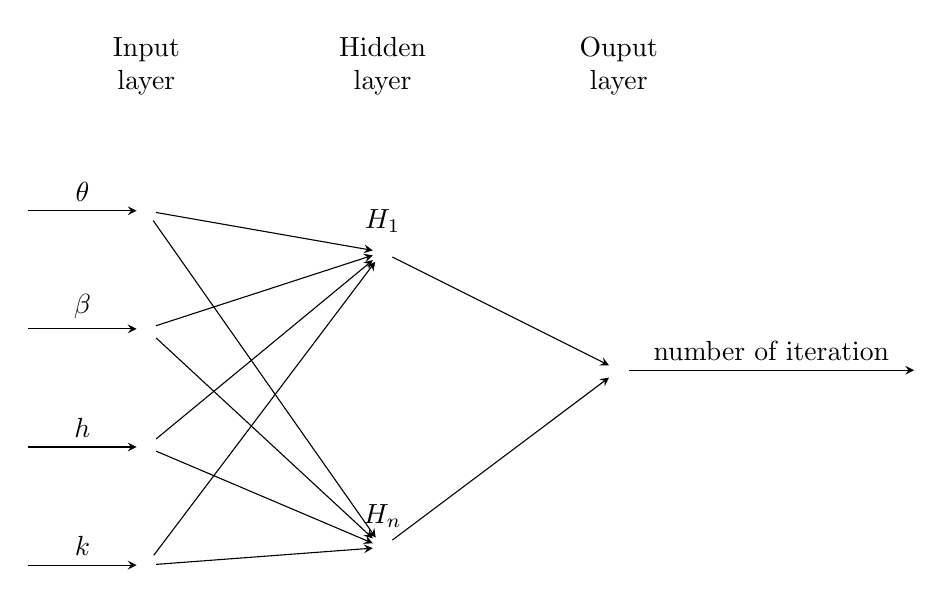
\begin{tikzpicture}[x=1.5cm, y=1.5cm, >=stealth]
\foreach \m/\l [count=\y] in {1,2,3,4}
  \node [every neuron/.try, neuron \m/.try] (input-\m) at (0,2.1-\y) {};

\foreach \m [count=\y] in {1,missing,2}
  \node [every neuron/.try, neuron \m/.try ] (hidden-\m) at (2,2-\y*1.25) {};

\foreach \m [count=\y] in {1}
  \node [every neuron/.try, neuron \m/.try ] (output-\m) at (4,0.75-\y) {};

\draw [<-] (input-1) -- ++(-1,0)
    node [above, midway] {$\theta$};
\draw [<-] (input-2) -- ++(-1,0)
    node [above, midway] {$\beta$};
\draw [<-] (input-3) -- ++(-1,0)
    node [above, midway] {$h$};
\draw [<-] (input-4) -- ++(-1,0)
    node [above, midway] {$k$};

%\foreach \l [count=\i] in {1,2,3,4}
%  \draw [<-] (input-\i) -- ++(-1,0)
%    node [above, midway] {$I_\l$};

\foreach \l [count=\i] in {1,n}
  \node [above] at (hidden-\i.north) {$H_\l$};

%\foreach \l [count=\i] in {1}
\draw [->] (output-1) -- ++(2.5,0)
    node [above, midway] {number of iteration};

\foreach \i in {1,...,4}
  \foreach \j in {1,...,2}
    \draw [->] (input-\i) -- (hidden-\j);

\foreach \i in {1,2}
  \foreach \j in {1}
    \draw [->] (hidden-\i) -- (output-\j);

\foreach \l [count=\x from 0] in {Input, Hidden, Ouput}
  \node [align=center, above] at (\x*2,2) {\l \\ layer};
\end{tikzpicture}
    \caption{Neural network architecture used for the elliptic problem with continuous exact solution. The number of hidden layers, $N_{hl}$, and the number of neuron for each hidden layer, $N_n$, are used as the sensitivity analysis parameters.}
    \label{fig:ell_ann_fig}
\end{figure}

Table \ref{table:ell_hyper_nl_nn_con} illustrates that the mean squared error of the validation set is generally decreased as $N_{hl}$ and $N_{n}$ are increased. The neural network performance, however, is not significantly improved when $N_{hl} > 2$ and $N_{n} > 80$. Hence, we select $N_{hl} = 2$ and $N_{n} = 80$ for the test set, and the $r^2$ and explained variance score is 0.98 and 0.98, respectively. These results illustrate the improvement of the prediction performance as the $r^2$ and explained variance score are improved from the multi-variable regression significantly.


\begin{table}[!ht]
\centering
\caption{Elliptic equation with continuous exact solution: Mean squared error of the validation set for different number of hidden layers $N_{hl}$ and different number of neurons per layer $N_{n}$}
\begin{tabular}{|c|c|c|c|c|}
\hline
\backslashbox{$N_{hl}$}{$N_n$}   & 10      & 20      & 40     & 80       \\ \hline

2     & 4.27  & 1.41  & 1.20  & 0.95 \\
    \hline
    4     & 2.21  & 1.43  & 2.13  & 1.58 \\
    \hline
    8     & 3.60  & 1.74  & 1.60  & 0.98 \\
    \hline

\end{tabular}
\label{table:ell_hyper_nl_nn_con}
\end{table}



\subsubsection{The effect of a type of exact solution and heterogeneous coefficient} Next, we investigate the effect of a type of exact solution, continuous and discontinous solutions, on the choice of optimal $\beta$ using different solvers and $\theta$ schemes. Moreover, $\boldsymbol{\kappa}$ is heterogeneous for both types of solution. For the continuous solution, we take $\Omega = \left[ 0,1\right]^2$ and choose the exact solution in $\Omega$ as:

\begin{equation}\label{eq:darcy_exact_solution_1}
p(x,y) := \sin(x+y),
\end{equation}

\noindent
which is similar to the previous section. However, $\boldsymbol{\kappa}$ is chosen as:

\begin{equation}\label{eq:darcy_exact_solution_1_kappa}
\boldsymbol{\kappa} := \kappa  \sin(x+y) \boldsymbol{I}.
\end{equation}

\noindent
Subsequently, $g$ is chosen as: 

\begin{equation}  \label{eq:darcy_source_1}
g(x,y) := 4.0 \kappa \sin(x+y) \cos(x+y).
\end{equation}

Next, for the discontinuous solution, we take $\Omega = \left[ 0,1\right]^1$ and choose the exact solution in $\Omega$ as:

\begin{equation}\label{eq:dis_exact_solution}
p =
\begin{cases}
%2.0x k_1/(k_0+k_1) \quad & \text { if } 0.0 < x \leq 0.5, \\
2.0x \frac{{\kappa}_1}{{\kappa}_0+{\kappa}_1} \quad & \text { if } x \leq 0.5, \\
\frac{\left( 2x-1 \right)  {\kappa}_0+{\kappa}_1}{{\kappa}_0+{\kappa}_1} \quad & \text { if } x > 0.5,
%0.0 \quad & \text { at } x = 0.0, \\
%1.0 \quad & \text { at } x = 1.0,
\end{cases}
\end{equation}

\noindent
where ${\kappa}_1$ and ${\kappa}_2$ represent multiplied coefficients for the $0 \leq x \leq 0.5$ and $1.0 \geq x > 0.5$ subdomains, respectively. ${\kappa}_1$ and ${\kappa}_2$ have the same range of $[1.0, 1.0 \times 10^{-18}]$ and ${\kappa}_1$ $\neq$ ${\kappa}_2$. Consequently, the $\boldsymbol{\kappa}$ for the discontinuous exact solution is read: 

\begin{equation}\label{eq:darcy_exact_solution_dis_kappa}
\boldsymbol{\kappa} :=
\begin{cases}
{\kappa}_1 \boldsymbol{I} \quad & \text { if }  0.0 \leq x \leq 0.5, \\
{\kappa}_2 \boldsymbol{I} \quad & \text { if }  1.0 \geq x > 0.5.
\end{cases}
\end{equation}

\noindent
Subsequently, the boundary conditions are applied as follows:

\begin{equation}\label{eq:dis_bound_solution}
p =
\begin{cases}
0.0 \quad & \text { at } x = 0.0, \\
1.0 \quad & \text { at } x = 1.0,
\end{cases}
\end{equation}

\noindent
We use Algorithm \ref{alg:ell_effect_of_k} where $k=1$ for each case, i.e. each case has different combination of solver, $\theta$, and the exact solutions. The results are shown in Table \ref{tab:ell_homo_beta_unstable_dis}. The results of SIPG illustrate the similarity between the continuous and discontinuous solutions. The results of IIPG, however, show a discrepancy as the lowest $\beta$ values that provides the optimal convergence rate solution are different between the continuous and discontinuous solutions. The type of solver, direct and iterative solvers, does not influence this value.


\begin{table}[h!]
  \centering
  \caption{The lowest $\beta$ value that provides the optimal convergence rate solution with different type of exact solution (continuous or discontinuous), $\theta$, and solver. Note that $\boldsymbol{{\kappa}}$ is heterogeneous, and $k=1$.}
    \begin{tabular}{|c|c|c|c|c|}
    \hline
    \multirow{2}[4]{*}{exact solution} & \multicolumn{2}{c|}{SIPG} & \multicolumn{2}{c|}{IIPG} \\
\cline{2-5}          & \multicolumn{1}{l|}{direct solver} & \multicolumn{1}{l|}{iterative solver} & \multicolumn{1}{l|}{direct solver} & \multicolumn{1}{l|}{iterative solver} \\
    \hline
    continuous & \multicolumn{1}{c|}{1.11} & \multicolumn{1}{c|}{1.11} & \multicolumn{1}{c|}{0.83} & \multicolumn{1}{c|}{0.83} \\
    \hline
    discontinuous & 1.11       &    1.11   &    0.89   & 0.89  \\
    \hline
    \end{tabular}%
  \label{tab:ell_homo_beta_unstable_dis}%
\end{table}%

Similar to the continuous solution, the choice of $\beta$ influences the number of linear iterative solver significantly, as illustrated in Figure \ref{fig:ell_het_noi}. In short, when $\beta$ is increased, the number of iteration increases, while the number of iteration increases sharply before the solution becomes unstable.

\begin{figure}[h!]
   \centering
        \includegraphics[width=6.0cm, height=6.0cm]{pictures/ell_homo_diff_k_sipg_it_sin.pdf}
        \includegraphics[width=6.0cm, height=6.0cm]{pictures/ell_homo_diff_k_iipg_it_sin.pdf}
        \includegraphics[width=6.0cm, height=6.0cm]{pictures/ell_homo_diff_k_sipg_it_dis.pdf}
        \includegraphics[width=6.0cm, height=6.0cm]{pictures/ell_homo_diff_k_iipg_it_dis.pdf}
   \caption{Number of linear iterative solver of cases which $\boldsymbol{{\kappa}}$ is heterogeneous and exact solution is continuous: (\textbf{a}) SIPG, (\textbf{b}) IIPG, $\boldsymbol{{\kappa}}$ is heterogeneous and exact solution is discontinuous: (\textbf{c}) SIPG, and (\textbf{d}) IIPG. Note that each line represents different value of ${\kappa}$ for the continuous solution, and ${\kappa}_1$ and ${\kappa}_2$ for the discontinuous solution. The error bar shows mean and standard derivation of each number of iteration.}
   \label{fig:ell_het_noi}
\end{figure}

Following the procedure, i.e. predicting the optimal $\beta$ for the iterative solver, used for the continuous solution, we firstly evaluate each independent variable using chi-squared test \cite{scikit-learn}. Its results are provided in Table \ref{tab:linear_regression_p_value_dis}, and this table shows that $\theta$ methods, $\beta$, and $h$ have a p-value less than 0.025. Hence, we include these variables as independent variables for a further predictive model development. 

\begin{table}[!ht]
  \centering
  \caption{Elliptic equation with discontinuous exact solution: p-value results for each explanatory variable}
    \begin{tabular}{|c|c|}
    \hline
    Variable & p-value \\
    \hline
    $\theta$ & $\approx$ 0.00 \\
    \hline
    $\kappa_0$  & $\approx$ 1.00 \\
    \hline
    $\kappa_1$      & $\approx$ 1.00 \\
    
    \hline
    $\beta$  & $\approx$ 0.00 \\
    \hline
    $h$     & $\approx$ 0.00 \\
    \hline
    
    \end{tabular}%
  \label{tab:linear_regression_p_value_dis}%
\end{table}%

We follow the same procedures, splitting technique and model development, as utilized in the previous model. The developed multi-variable regression \cite{scikit-learn} is read:

\begin{equation} \label{eq:ell_regression_dis}
\begin{split}
\mathrm{number \ of \ iteration} = \alpha 
    &+ \gamma_{1} \times \theta \\
    &+ \gamma_{2} \times \beta    \\
    &+ \gamma_{3} \times h 
\end{split}
\end{equation}

\noindent
where $\alpha = 19.59$, $\gamma_{1} = -0.86$, $\gamma_{2} = 0.42$, and $\gamma_{3} = -19.51$. The $r^2$ and explained variance score is 0.84 and 0.84, respectively.

Next, we develop ANN model using three input and one output as shown in Figure \ref{fig:ell_ann_fig_dis} and use number of hidden layer ($n_{hl}$) and number of neuron ($n_n$) for hyper-parameter tuning. ReLU is used as an activation function for each neuron of the hidden layer.

\tikzset{%
  every neuron/.style={
    circle,
    draw,
    minimum size=1cm
  },
  neuron missing/.style={
    draw=none, 
    scale=4,
    text height=0.333cm,
    execute at begin node=\color{black}$\vdots$
  },
}
\begin{figure}
    \centering
    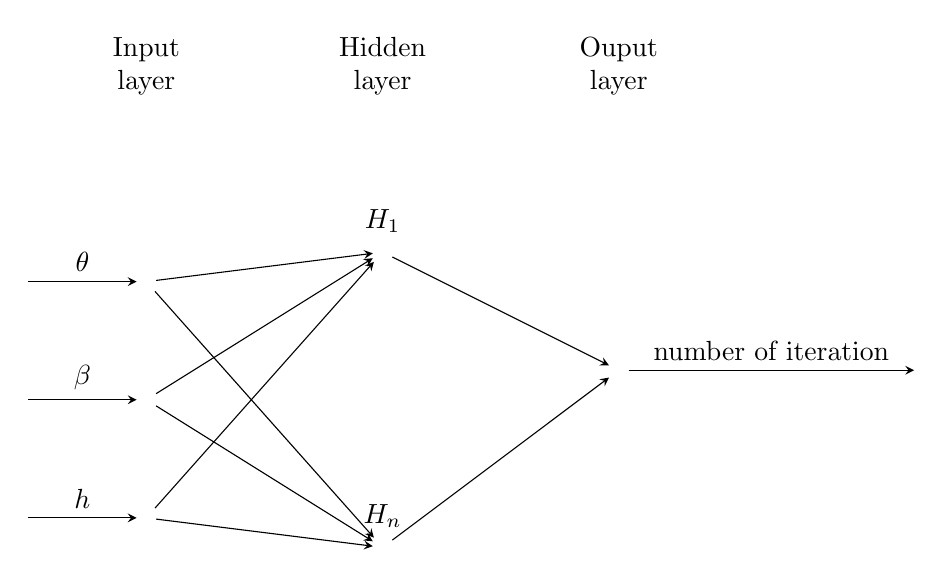
\begin{tikzpicture}[x=1.5cm, y=1.5cm, >=stealth]
\foreach \m/\l [count=\y] in {1,2,3}
  \node [every neuron/.try, neuron \m/.try] (input-\m) at (0,1.5-\y) {};

\foreach \m [count=\y] in {1,missing,2}
  \node [every neuron/.try, neuron \m/.try ] (hidden-\m) at (2,2-\y*1.25) {};

\foreach \m [count=\y] in {1}
  \node [every neuron/.try, neuron \m/.try ] (output-\m) at (4,0.75-\y) {};

\draw [<-] (input-1) -- ++(-1,0)
    node [above, midway] {$\theta$};
\draw [<-] (input-2) -- ++(-1,0)
    node [above, midway] {$\beta$};
\draw [<-] (input-3) -- ++(-1,0)
    node [above, midway] {$h$};

%\foreach \l [count=\i] in {1,2,3,4}
%  \draw [<-] (input-\i) -- ++(-1,0)
%    node [above, midway] {$I_\l$};

\foreach \l [count=\i] in {1,n}
  \node [above] at (hidden-\i.north) {$H_\l$};

%\foreach \l [count=\i] in {1}
\draw [->] (output-1) -- ++(2.5,0)
    node [above, midway] {number of iteration};

\foreach \i in {1,...,3}
  \foreach \j in {1,...,2}
    \draw [->] (input-\i) -- (hidden-\j);

\foreach \i in {1,2}
  \foreach \j in {1}
    \draw [->] (hidden-\i) -- (output-\j);

\foreach \l [count=\x from 0] in {Input, Hidden, Ouput}
  \node [align=center, above] at (\x*2,2) {\l \\ layer};
\end{tikzpicture}
    \caption{Neural network architecture used for the elliptic problem with discontinuous exact solution. The number of hidden layers, $N_{hl}$, and the number of neuron for each hidden layer, $N_n$, are used as the sensitivity analysis parameters.}
    \label{fig:ell_ann_fig_dis}
\end{figure}

Table \ref{table:ell_hyper_nl_nn_dis} presents that the mean squared error of the validation set is decreased, as expected, as $N_{hl}$ and $N_{n}$ are increased. We select $N_{hl} = 2$ and $N_{n} = 80$ for the test set, and the $r^2$ and explained variance score is 0.98 and 0.98, respectively. The neural network outperforms the multi-variable regression.

\begin{table}[!ht]
\centering
\caption{Elliptic equation with discontinuous exact solution: Mean squared error of the validation set for different number of hidden layers $N_{hl}$ and different number of neurons per layer $N_{n}$}
\begin{tabular}{|c|c|c|c|c|}
\hline
\backslashbox{$N_{hl}$}{$N_n$}   & 10      & 20      & 40     & 80       \\ \hline

2     & 5.49  & 1.57  & 3.16  & 1.67 \\
    \hline
    4     & 1.93  & 1.53  & 1.71  & 1.63 \\
    \hline
    8     & 1.44  & 2.34  & 1.43  & 1.56 \\
    \hline

\end{tabular}
\label{table:ell_hyper_nl_nn_dis}
\end{table}



\subsection{Biot's equations}

TODO add oscillation examples

\begin{equation}\label{eq:biot_kappa}
\boldsymbol{\kappa} :=
\begin{cases}
{\kappa}_1 \boldsymbol{I} \quad & \text { if }  0.0 \leq x \leq 0.5, \\
{\kappa}_2 \boldsymbol{I} \quad & \text { if }  1.0 \geq x > 0.5, \\
\end{cases} \\
\end{equation}

\noindent
and

\begin{equation}\label{eq:k_mult}
\kappa_{mult} = \frac{{\kappa}_2 }{{\kappa}_1 }
\end{equation}

\begin{algorithm}[!ht]
\caption{Investigation procedure for the Biot's equations}
\label{alg:biot_procedure}
\begin{algorithmic}
%\STATE{Initialize the set of $\boldsymbol{\kappa}$ that used in the investigation}
%\STATE{Initialize the set of $\kappa_{mult}$ that used in the investigation}
%\STATE{Initialize the set of $h$ that used in the investigation}
%\STATE{Initialize the set of $\beta$ that used in the investigation}
\STATE{Initialize: sets of each variables; $\boldsymbol{\kappa}$, $\kappa_{mult}$, $h$, and  $\beta$}
\STATE{Initialize the result vector with \textsc{bool} solution quality}
\COMMENT{solution quality; 0 - Good and 1 - Bad}

\FOR{$i$ $<$ $n_{\boldsymbol{\kappa}}$, where $n_{\boldsymbol{\kappa}}$ is the size of the specified $\boldsymbol{\kappa}$ list}

\STATE{Assign $\boldsymbol{\kappa}_1:=\boldsymbol{\kappa}\left[i\right]$}

\FOR{$j$ $<$ $n_{\kappa_{mult}}$, where $n_{\kappa_{mult}}$ is the size of the specified $\kappa_{mult}$ list}

\STATE{Assign $\boldsymbol{\kappa}_2:=\kappa_{mult}\left[j\right] \times \boldsymbol{\kappa}_1$}

\FOR{$k$ $<$ $n_h$, where $n_h$ is the size of the specified $h$ list}

\STATE{Assign $h:=h\left[k\right]$}

\FOR{$l$ $<$ $n_{\beta}$, where $n_{\beta}$ is the size of the specified $\beta$ list}

\STATE{Assign $\beta:=\beta\left[l\right]$}
\STATE{Perform simulation}

\IF{Solution is stable} 
\IF{Solution exhibits nonphysical oscillation} 
\STATE{Assign 1 -$>$ result}
\ELSE 
\STATE{Assign 0 -$>$ result}
\ENDIF
\ELSE 
\STATE{Assign 1 -$>$ result}
\ENDIF
\ENDFOR
\ENDFOR
\ENDFOR
\ENDFOR
\end{algorithmic}
\end{algorithm}


\begin{table}[!ht]
  \centering
  \caption{Biot's equations: p-value results for each explanatory variable}
    \begin{tabular}{|c|c|}
    \hline
    Variable & p-value \\
    \hline
    $\boldsymbol{\kappa}_1$ & $\approx$ 0.00 \\
    \hline
    $\boldsymbol{\kappa}_2$ & $\approx$ 0.00 \\
    \hline
    $\kappa_{mult}$ & $\approx$ 0.00 \\
    \hline
    $\beta$  & $\approx$ 0.00 \\
    \hline
    $h$     & $\approx$ 0.01 \\
    \hline
    \end{tabular}%
  \label{tab:linear_regression_p_value_biot}%
\end{table}%


\begin{equation} \label{eq:biot_regression_dis}
\begin{split}
log\left(\frac{p(\mathbb{O}=1)}{1-(p(\mathbb{O}=1))}\right) = \alpha 
    &+ \gamma_{1} \times \boldsymbol{\kappa}_1 \\
    &+ \gamma_{2} \times \boldsymbol{\kappa}_2 \\
    &+ \gamma_{3} \times \kappa_{mult} \\
    &+ \gamma_{4} \times \beta    \\
    &+ \gamma_{5} \times h 
\end{split}
\end{equation}

\noindent
and

\begin{equation}\label{eq:exact_solution}
\mathbb{O}=
\begin{cases}
1, & \text{if} \ p(\mathbb{O}=1) \ge 0.5 \\
0, & \text{if} \ p(\mathbb{O}=1) < 0.5
\end{cases}
\end{equation}

\noindent
where $\alpha = -1.19$, $\gamma_{1} = -0.06$, , $\gamma_{2} = 0.68$, $\gamma_{3} = 5.55$, $\gamma_{4} = -5.49$, and $\gamma_{5} = 0.32$. The accuracy of the logistic regression model is 0.80.



\begin{table}[!ht]
  \centering
  \caption{Biot's equations: Confusion matrix of the logistic regression for the test set}
    \begin{tabular}{|c|c|c|c|}
    \hline
    \multicolumn{2}{|c|}{\multirow{2}[4]{*}{total test set = 1415}} & \multicolumn{2}{c|}{Test set values} \\
\cline{3-4}    \multicolumn{2}{|c|}{} & \multicolumn{1}{l|}{Positive (1)} & \multicolumn{1}{l|}{Negative (0)} \\
    \hline
    \multirow{2}[4]{*}{Predicted values} & Positive (1) & 959   & 74 \\
\cline{2-4}          & Negative (0) & 210   & 172 \\
    \hline
    \end{tabular}%
  \label{tab:biot_cm_logistic}%
\end{table}%

\tikzset{%
  every neuron/.style={
    circle,
    draw,
    minimum size=1cm
  },
  neuron missing/.style={
    draw=none, 
    scale=4,
    text height=0.333cm,
    execute at begin node=\color{black}$\vdots$
  },
}
\begin{figure}
    \centering
    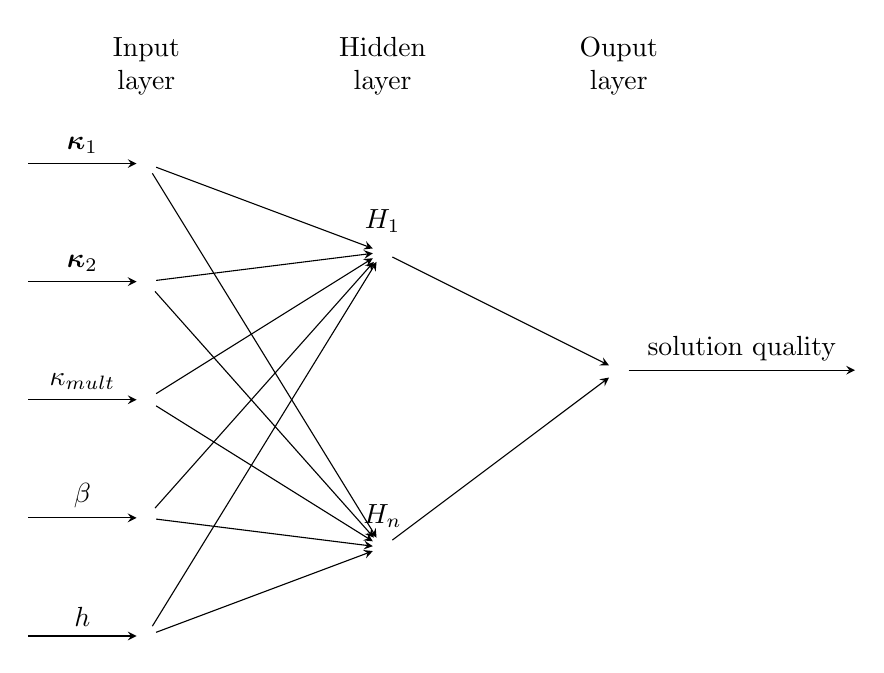
\begin{tikzpicture}[x=1.5cm, y=1.5cm, >=stealth]
\foreach \m/\l [count=\y] in {1,2,3,4,5}
  \node [every neuron/.try, neuron \m/.try] (input-\m) at (0,2.5-\y) {};

\foreach \m [count=\y] in {1,missing,2}
  \node [every neuron/.try, neuron \m/.try ] (hidden-\m) at (2,2-\y*1.25) {};

\foreach \m [count=\y] in {1}
  \node [every neuron/.try, neuron \m/.try ] (output-\m) at (4,0.75-\y) {};

\draw [<-] (input-1) -- ++(-1,0)
    node [above, midway] {$\boldsymbol{\kappa}_1$};
\draw [<-] (input-2) -- ++(-1,0)
    node [above, midway] {$\boldsymbol{\kappa}_2$};
\draw [<-] (input-3) -- ++(-1,0)
    node [above, midway] {$\kappa_{mult}$};
\draw [<-] (input-4) -- ++(-1,0)
    node [above, midway] {$\beta$};
\draw [<-] (input-5) -- ++(-1,0)
    node [above, midway] {$h$};

%\foreach \l [count=\i] in {1,2,3,4}
%  \draw [<-] (input-\i) -- ++(-1,0)
%    node [above, midway] {$I_\l$};

\foreach \l [count=\i] in {1,n}
  \node [above] at (hidden-\i.north) {$H_\l$};

%\foreach \l [count=\i] in {1}
\draw [->] (output-1) -- ++(2.,0)
    node [above, midway] {solution quality};

\foreach \i in {1,...,5}
  \foreach \j in {1,...,2}
    \draw [->] (input-\i) -- (hidden-\j);

\foreach \i in {1,2}
  \foreach \j in {1}
    \draw [->] (hidden-\i) -- (output-\j);

\foreach \l [count=\x from 0] in {Input, Hidden, Ouput}
  \node [align=center, above] at (\x*2,2) {\l \\ layer};
\end{tikzpicture}
    \caption{Neural network architecture used for the Biot's equation. The number of hidden layers, $N_{hl}$, and the number of neuron for each hidden layer, $N_n$, are used as the sensitivity analysis parameters.}
    \label{fig:biot_ann_fig}
\end{figure}

\begin{table}[!ht]
\centering
\caption{Biot's equations: Accuracy of the validation set for different number of hidden layers $N_{hl}$ and different number of neurons per layer $N_{n}$}
\begin{tabular}{|c|c|c|c|c|c|}
\hline
\backslashbox{$N_{hl}$}{$N_n$}   & 10      & 20      & 40     & 80   & 120     \\ \hline

    2     & 0.89  & 0.93  & 0.93  & 0.93  & 0.92 \\
    \hline
    4     & 0.89  & 0.93  & 0.93  & 0.93  & 0.93 \\
    \hline
    8     & 0.88  & 0.92  & 0.93  & 0.93  & 0.93 \\
    \hline
    16    & 0.73  & 0.73  & 0.73  & 0.27  & 0.27 \\
    \hline
    32    & 0.73  & 0.73  & 0.73  & 0.73  & 0.73 \\
    \hline

\end{tabular}
\label{table:biot_hyper_nl_nn_dis}
\end{table}

The accuracy of the ANN using the test set is 0.93.

\begin{table}[!ht]
  \centering
  \caption{Biot's equations: Confusion matrix of the artificial neural network (ANN) for the test set}
    \begin{tabular}{|c|c|c|c|}
    \hline
    \multicolumn{2}{|c|}{\multirow{2}[4]{*}{total test set = 1415}} & \multicolumn{2}{c|}{Test set values} \\
\cline{3-4}    \multicolumn{2}{|c|}{} & \multicolumn{1}{l|}{Positive (1)} & \multicolumn{1}{l|}{Negative (0)} \\
    \hline
    \multirow{2}[4]{*}{Predicted values} & Positive (1) & 961   & 72 \\
\cline{2-4}          & Negative (0) & 15    & 367 \\
    \hline
    \end{tabular}%
  \label{tab:biot_cm_ann}%
\end{table}%

Conclusion
\begin{itemize}
\item For Darcy with smooth coefficients : need a minimum $\beta$ but not the maximum for optimal convergence rate. However, the iterative solver is affected.
\item For Darcy with non-smooth coefficients : To observe sub-optimal convergence rate, minimum and maximum bound for $\beta$ is required. 
\item For Biot's equations : to avoid oscillations, optimal choice of $\beta$ is required. Here we employ SIPG and iterative solver. 
\end{itemize}

\section{Conclusions}
\label{sec:conclusions}

Some conclusions here.



\section*{Acknowledgments}
We would like to acknowledge the assistance of volunteers in putting
together this example manuscript and supplement.

\bibliographystyle{siamplain}
\bibliography{lit}
\end{document}
